\chapter{Transfer procedure of monolayer TMDCs from the native substrate to $SiO_2/Si$ wafer}
\label{cha:Transfer}
\section{Introduction}
The most common method of producing the TMDCs is CVD. During the CVD growth the process the substrate and the sample are heated to very high temperatures, up to 1000 {\degree}C. Because of that there is substantial thermal expansion in both substrate and sample. However due to difference in thermal expansion coefficient between those two elements there is potential build up of thermal strain. Additionally because the substrate, upon which the sample is grown, is heated to such high temperatures that it cannot be used for electrical measurements. More specifically the thermal expansion coefficients of $WS_2$ and $SiO_2$ are on the order of $10^{-3}$ and $10^{-7}$ $K^{-1}$ respectively \cite{Hu2018}\cite{Tada2000}. Therefore it is expected that during cooling down the $WS_2$ will come under tension due to thermal expansion coefficient misalignment. There has been studies showing variation in PL position and FWHM under strain \cite{Aslan2018}. Similarly Raman peaks have also been shown to become shifted under strain, especially when using polarised light source \cite{Dadgar2018}. Theoretical studies have also shown effect of change in lattice constants on electronic band structure of TMDCs \cite{Yun2012}. Moreover in order to use TMDCs as components in devices different layers have to arranged together either vertically or laterally. Due to aforementioned reasons there is a need to develop methods for transferring single layers of TDMCs from one substrate to another one. In this chapter a focus is put on transferring $WS_2$ monolayer flakes from $SiO_2/Si$ onto other surfaces.
		
\section{Experimental}
		
The most common method of transferring flakes synthesised via CVD method is a wet transfer method utilising as an intermediate substrate. In such procedure a thin layer of PMMA is first spun on top of the substrate. After drying the substrate is placed in a KOH aqueous solution (6\% to 8\%) heated to about 50 {\degree}C. As a result the thin layer of $SiO_2$ on top of $Si$ is dissolved leaving a PMMA with the sample attached to it floating on top of the solution. The PMMA is then rinsed in water several times and scooped up onto a new substrate. Next the sample is dried and annealed to ensure good adhesion and remove wrinkles and strain. Then the PMMA is removed with a solution of acetone and IPA at about 50 {\degree}C. Any remaining PMMA can be removed by annealing the sample at about 100 {\degree}C.  
		
\section{Results}
	
A sample has been investigated using Raman and PL spectroscopy before and after transfer. In Figure \ref{fig:TransferPLMapsComparison} a comparison between samples before and after transfer can be seen in PL spectra. The as grown sample shows mostly homogeneous PL intensity, position and FWHM across the sample with the exception of the edge and trisecting lines in the middle where the PL intensity is higher and lower accordingly. In the sample after transfer the PL intensity, position and FWHM is more randomly distributed across the flake and there is a distinct lack of edge enhancement or the presence of trisecting lines.
	
The position of the PL peak from the as grown sample is $1.97 \pm (9.84 \times 10^{-4})$ eV, while the PL peak position from transferred sample $1.97 \pm (8.35 \times 10^{-3})$ eV. Therefore the peak position is shifted by 6.2 meV after transfer while the relative standard deviation is about 8.5 times greater in the transferred sample than in the as grown sample. The FWHM in the as grown sample is $36.37 \pm 0.79$ meV while in the transferred sample the FWHM is $83.27 \pm 6.79$ meV. The FWHM then increases by 46.90 meV while the relative standard deviation increases 3.72 times compared to the as grown sample.

The Raman $E^1_{2g}$ peak position in the as grown sample is $350.87 \pm 0.21$ $cm^{-1}$ while in the transferred sample is $351.34 \pm 0.29$ $cm^{-1}$. The relative uncertainty is therefore 1.39 greater in the transferred sample. The position of the Raman $A_{1g}$ peak in the as grown sample is $418.65 \pm 0.28$ $cm^{-1}$ while in the transferred sample it is $417.32 \pm 0.48$ $cm^{-1}$ . The relative uncertainty is therefore $1.69$ times greater in the transferred sample. The position difference between these two peaks is $67.79 \pm 0.24$ $cm^{-1}$ in the as grown sample while it is $66.01 \pm 0.48$ $cm^{-1}$ in the transferred sample. The relative uncertainty increases therefore by $2.03$ after the transfer. The intensity ratio between those peaks in the as grown sample is $5.75 \pm 0.68$ and after transfer it is $7.16 \pm 0.89$. The relative uncertainty changes $1.58$ times after transfer.
	
It can be therefore seen that after transfer the relative uncertainty increases for every parameter of Raman and PL spectra maps. This indicates that the sample after the transfer is much less homogeneous. Because both the position of PL as well as the position of Raman peaks is affected by the strain the inhomogeneity can indicate a relaxation or build up of strain. Since the CVD growth method involves heating up the sample and the substrate to very high temperatures, up to $850 {\degree}C$, there is possibility of residual thermal strain after cooling down. Since the PMMA is much more flexible than the $SiO_2$, that the sample is grown on, the $WS_2$ can relax before being placed on a new $SiO_2$ substrate. On the other hand the water present in between the $WS_2$ and PMMA can also be a source of strain. During the water evaporation the surface tension can induce local strain leading to high inhomogeneity. The PMMA can also have varying thickness and can swell to small degree therefore contracting in size during drying. Any or all of these effects can potentially contribute to the variation in parameters observed.
	
The average values of peak fitting parameters can be then compared between the two sample states to estimate the strain in the sample. The average position of $E^1_{2g} + 2LA$ peak changes from 350.8601 $cm^{-1}$ to 351.34 $cm^{-1}$, a 0.48 $cm^{-1}$ difference. Since the position of this peak changes by -3.1 $cm^{-1} / \%$ this indicates the change in strain of -0.16$\%$. The $E^1_{2g} + 2LA$ peak intensity change ($\Delta I / I_0$) of 23.15$\%$ indicates a 0.23$\%$ change in strain. The average value of $A_{1g}$ peak position changes from 418.65 $cm^{-1}$ to 417.32 $cm^{-1}$, a difference of 1.33 $cm^{-1}$. This indicates then a strain of -4.45$\%$. The intensity change of $A_{1g}$ peak of 25.64$\%$ corresponds to 0.33$\%$ strain \cite{Dadgar2018}.
	
The PL peak position changes from 1.9765 eV to 1.9703 which corresponds to change from about 1$\%$ to 0.75$\%$ strain, a -0.25$\%$ change \cite{Aslan2018}.
	
By comparing different average Raman and PL peaks fit parameters it is not clear to what extent the $WS_2$ is strained before or after the transfer. Neither the direction nor the extent of strain can be estimated then in the sample overall. The difference in deviation of theses values however indicates that the sample after transfer is less homogeneous than before. Therefore while it cannot be said that the sample strain changes on average as a whole, there is a change in strain across the sample. While the thermal strain should result in the sample as a whole being under tension due to thermal expansion and contraction other effects could still take place like aforementioned variation in water presence, inhomogeneity of PMMA layer thickness or folds in PMMA layer.
	
\begin{figure}[H] %PL Transfer Maps
	\begin{center}
		\begin{subfigure}[b]{0.4\textwidth}
			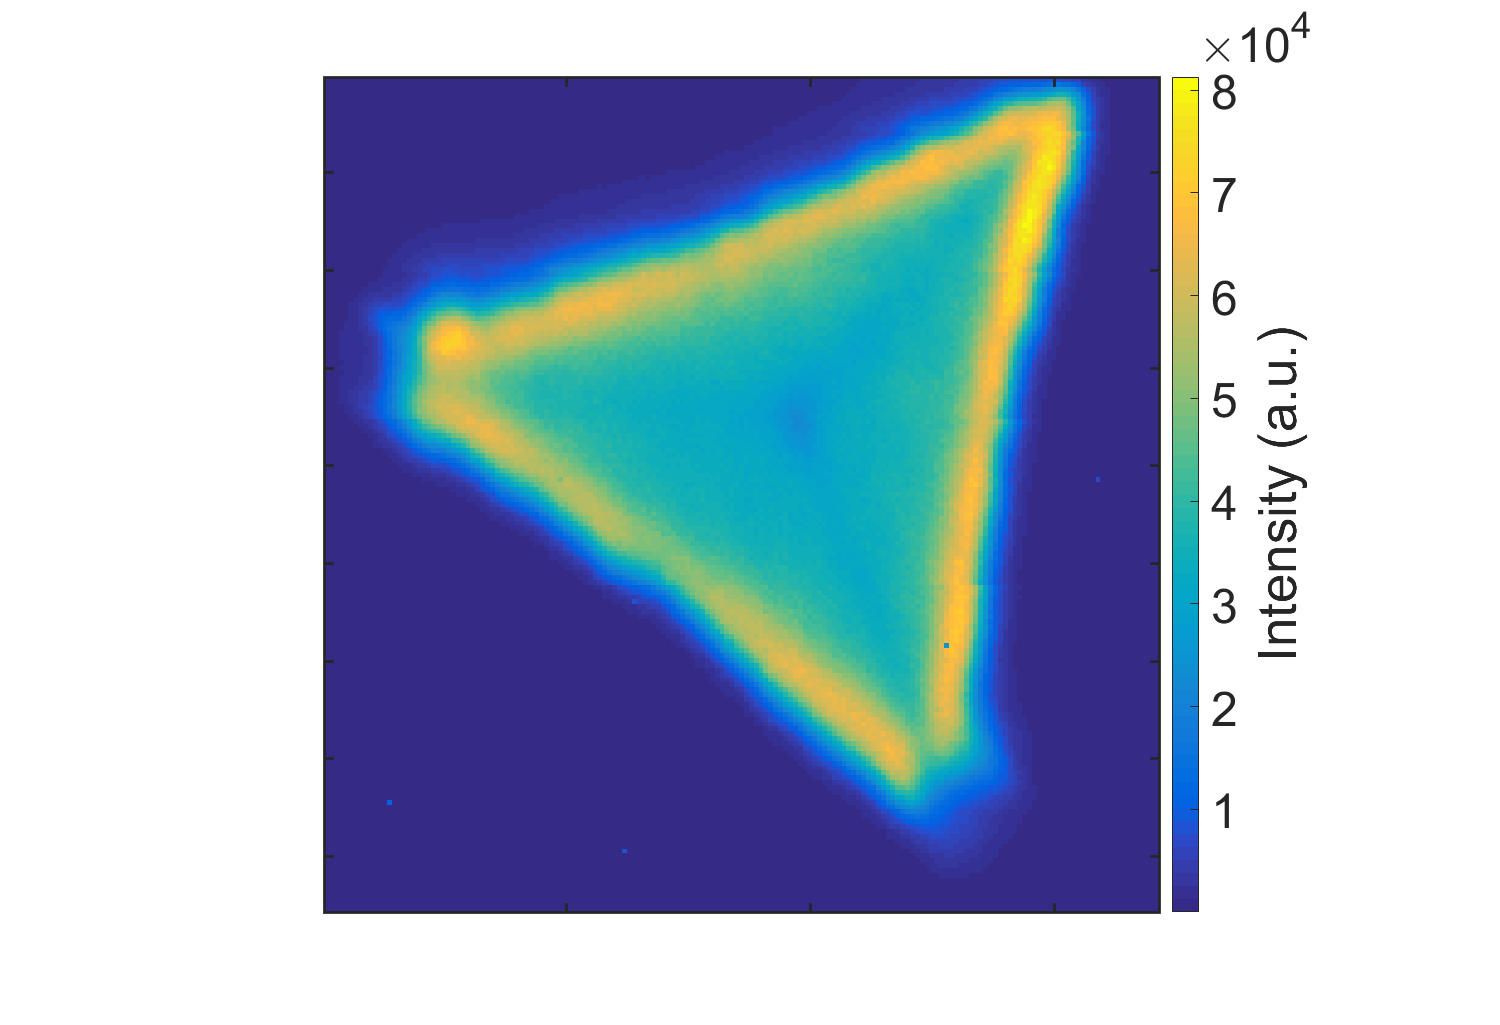
\includegraphics[scale=0.15]{Transfer/TransferPLIntensityMapAsgrown.png}
			\caption{PL Intensity map of as grown sample}
			\label{fig:TransferPLIntensityMapAsgrown}
		\end{subfigure}
		\quad
		\begin{subfigure}[b]{0.4\textwidth}
			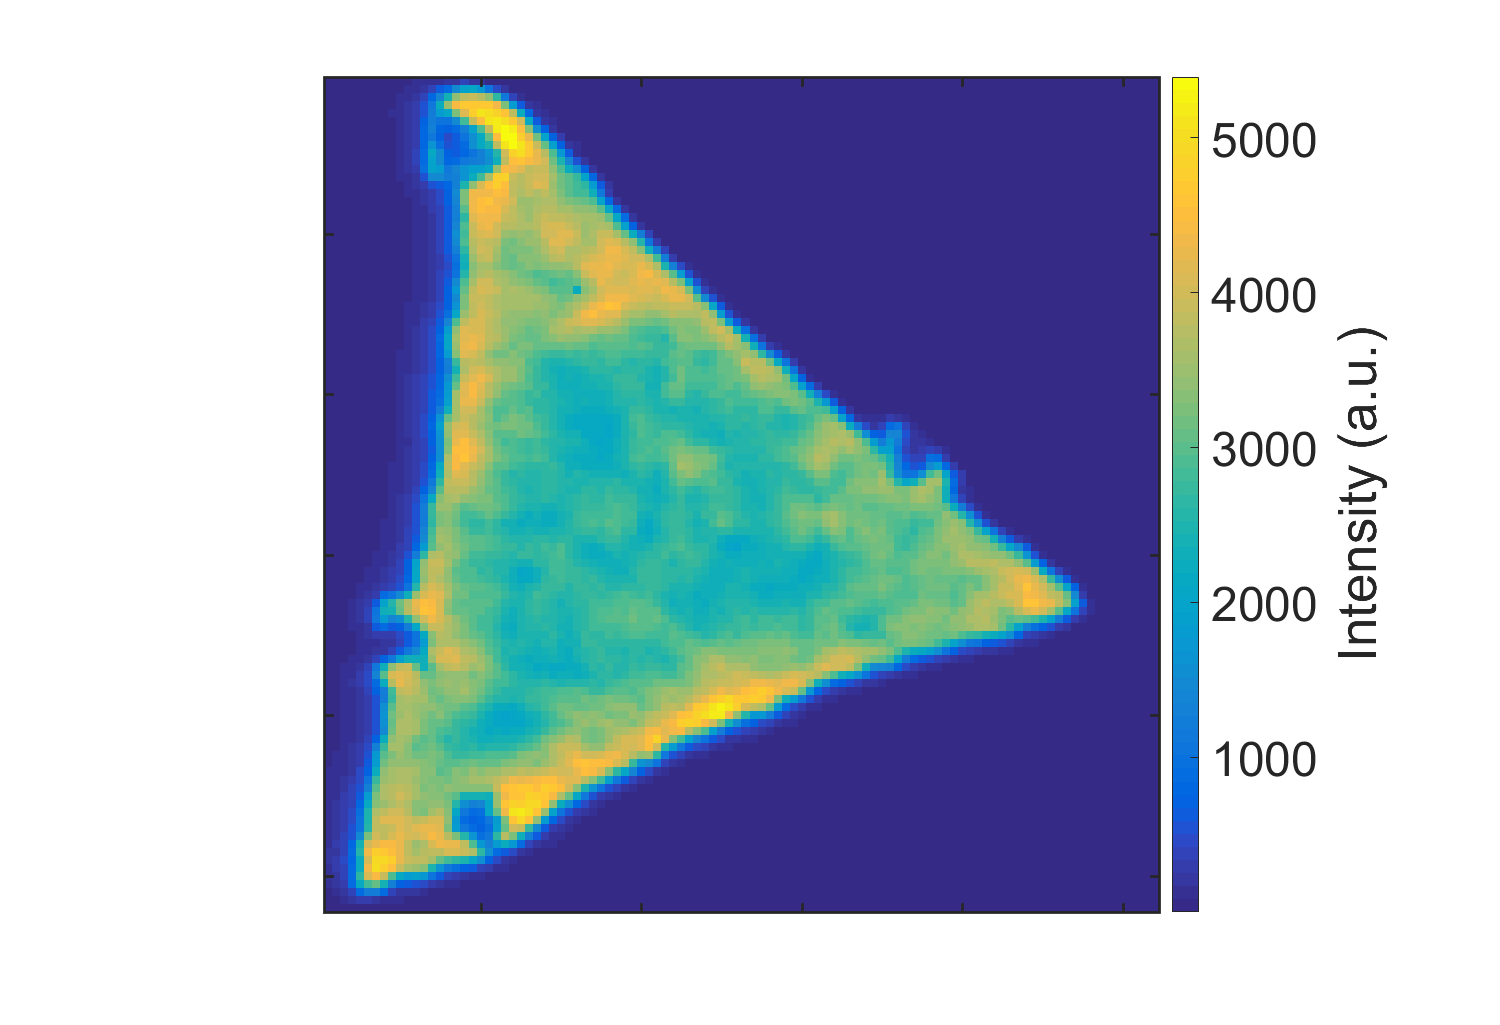
\includegraphics[scale=0.15]{Transfer/TransferPLIntensityMapTransferred.png}
			\caption{PL Intensity map of transferred sample}
			\label{fig:TransferPLIntensityMapTransferred}
		\end{subfigure}
		\vfill
		\begin{subfigure}[b]{0.4\textwidth}
			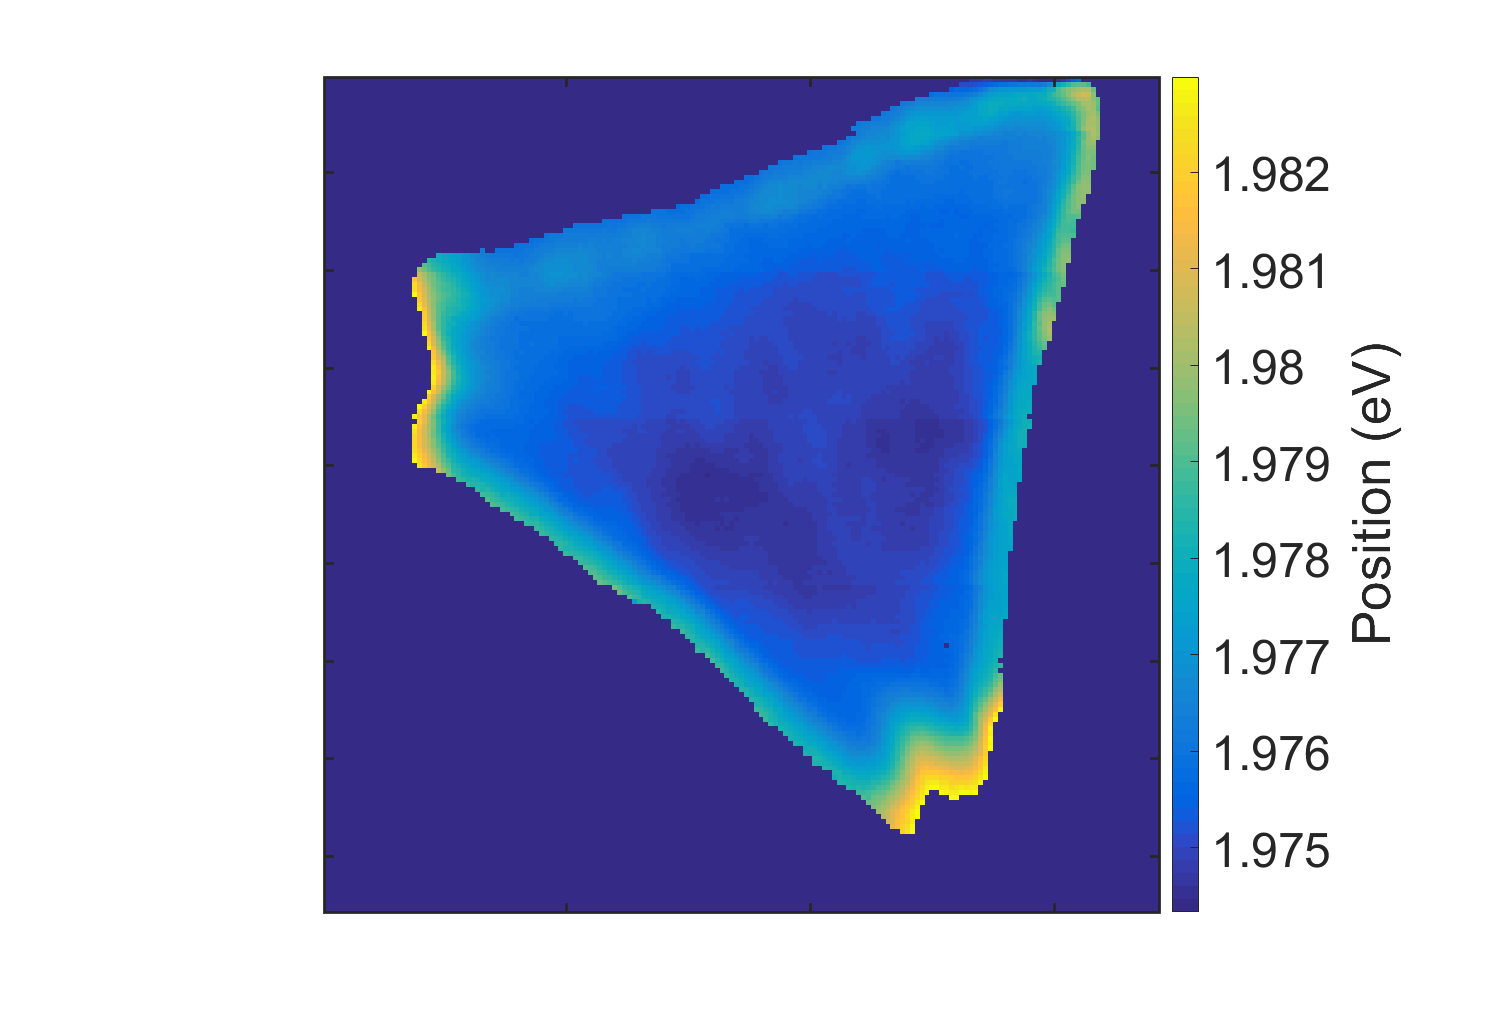
\includegraphics[scale=0.15]{Transfer/TransferPLPositionMapAsgrown.png}
			\caption{PL Position map of as grown sample}
			\label{fig:TransferPLPositionMapAsgrown}
		\end{subfigure}
		\quad
		\begin{subfigure}[b]{0.4\textwidth}
			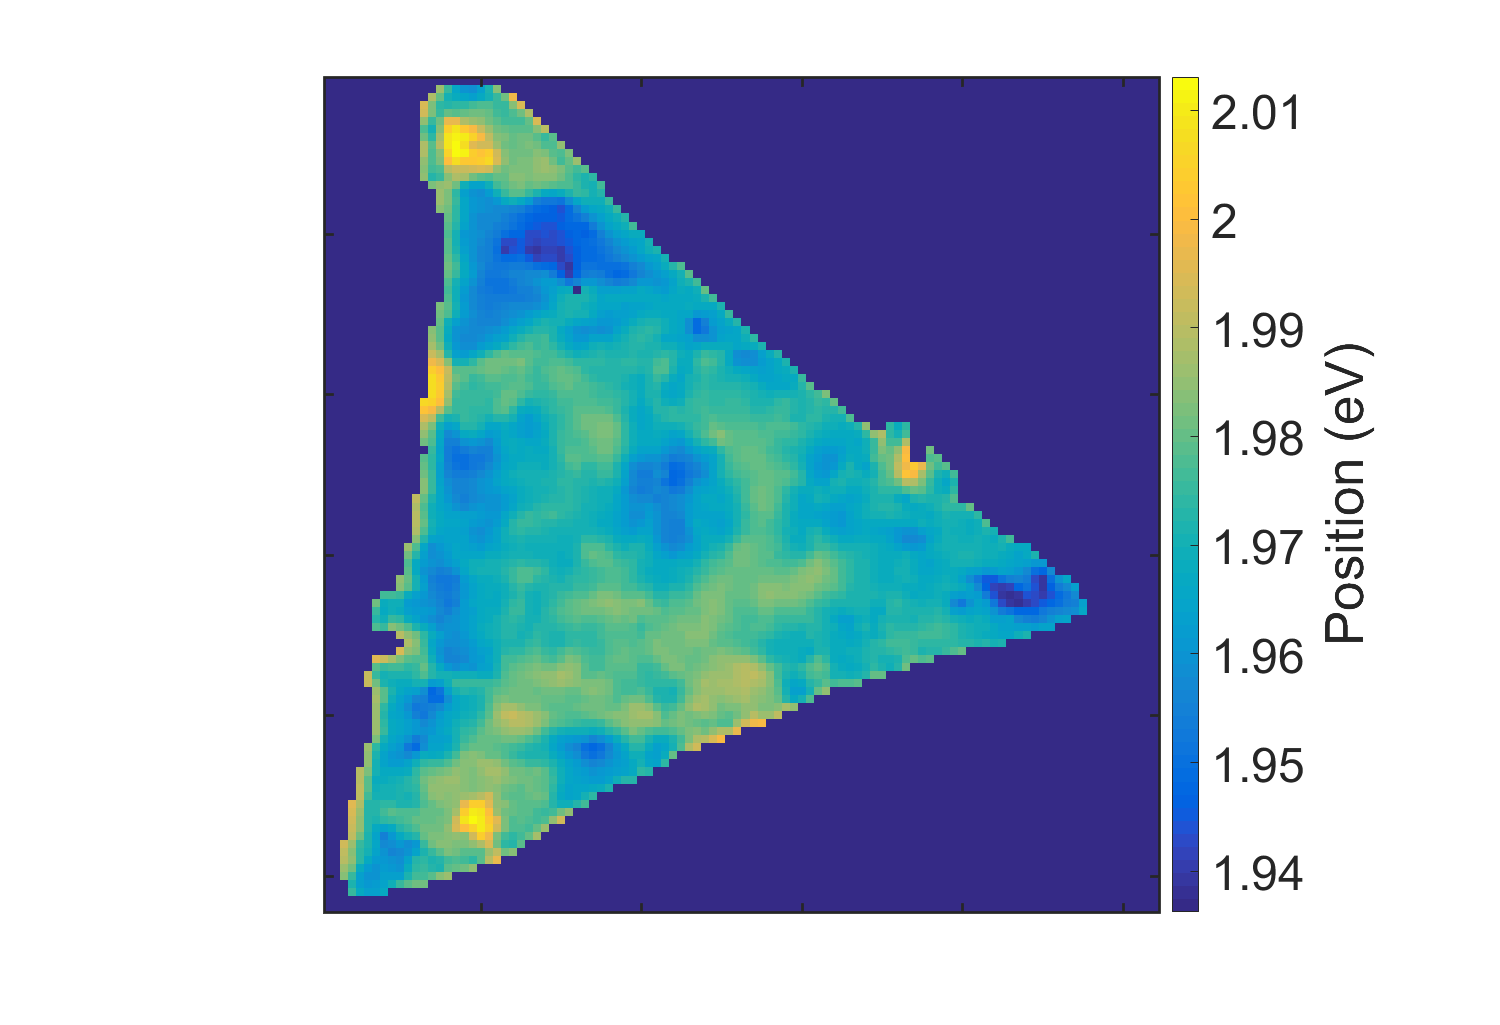
\includegraphics[scale=0.15]{Transfer/TransferPLPositionMapTransferred.png}
			\caption{PL Position map of transferred sample}
			\label{fig:TransferPLPositionMapTransferred}
		\end{subfigure}
		\vfill
		\begin{subfigure}[b]{0.4\textwidth}
			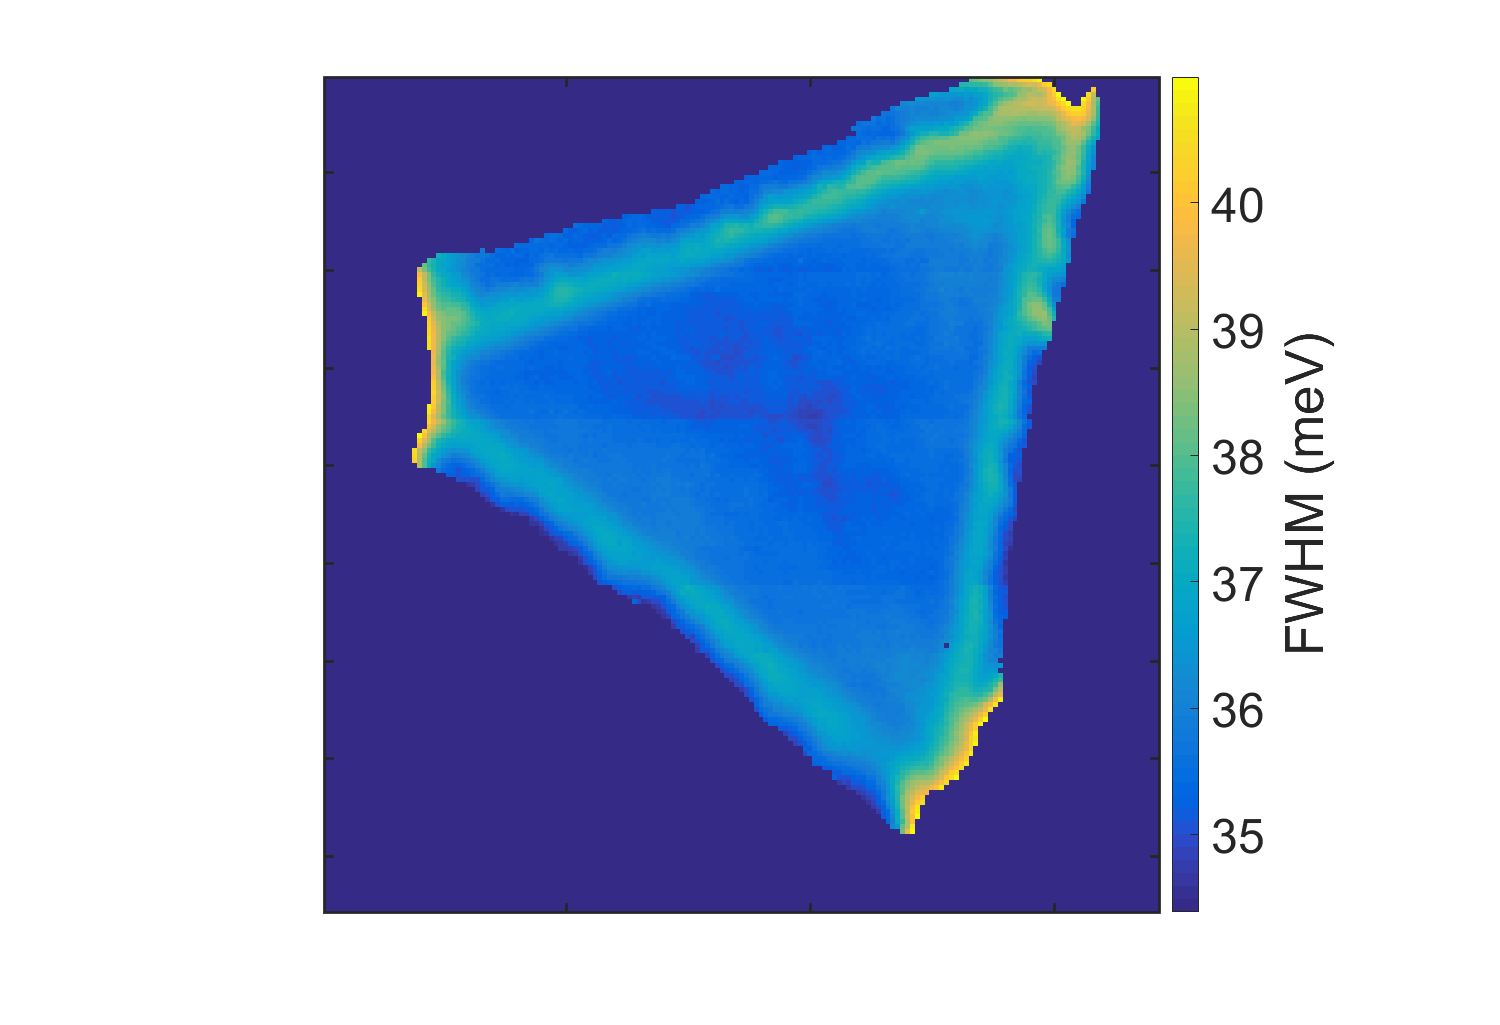
\includegraphics[scale=0.15]{Transfer/TransferPLWidthMapAsgrown.png}
			\caption{PL FWHM map of as grown sample}
			\label{fig:TransferPLWidthMapAsgrown}
		\end{subfigure}
		\quad
		\begin{subfigure}[b]{0.4\textwidth}
			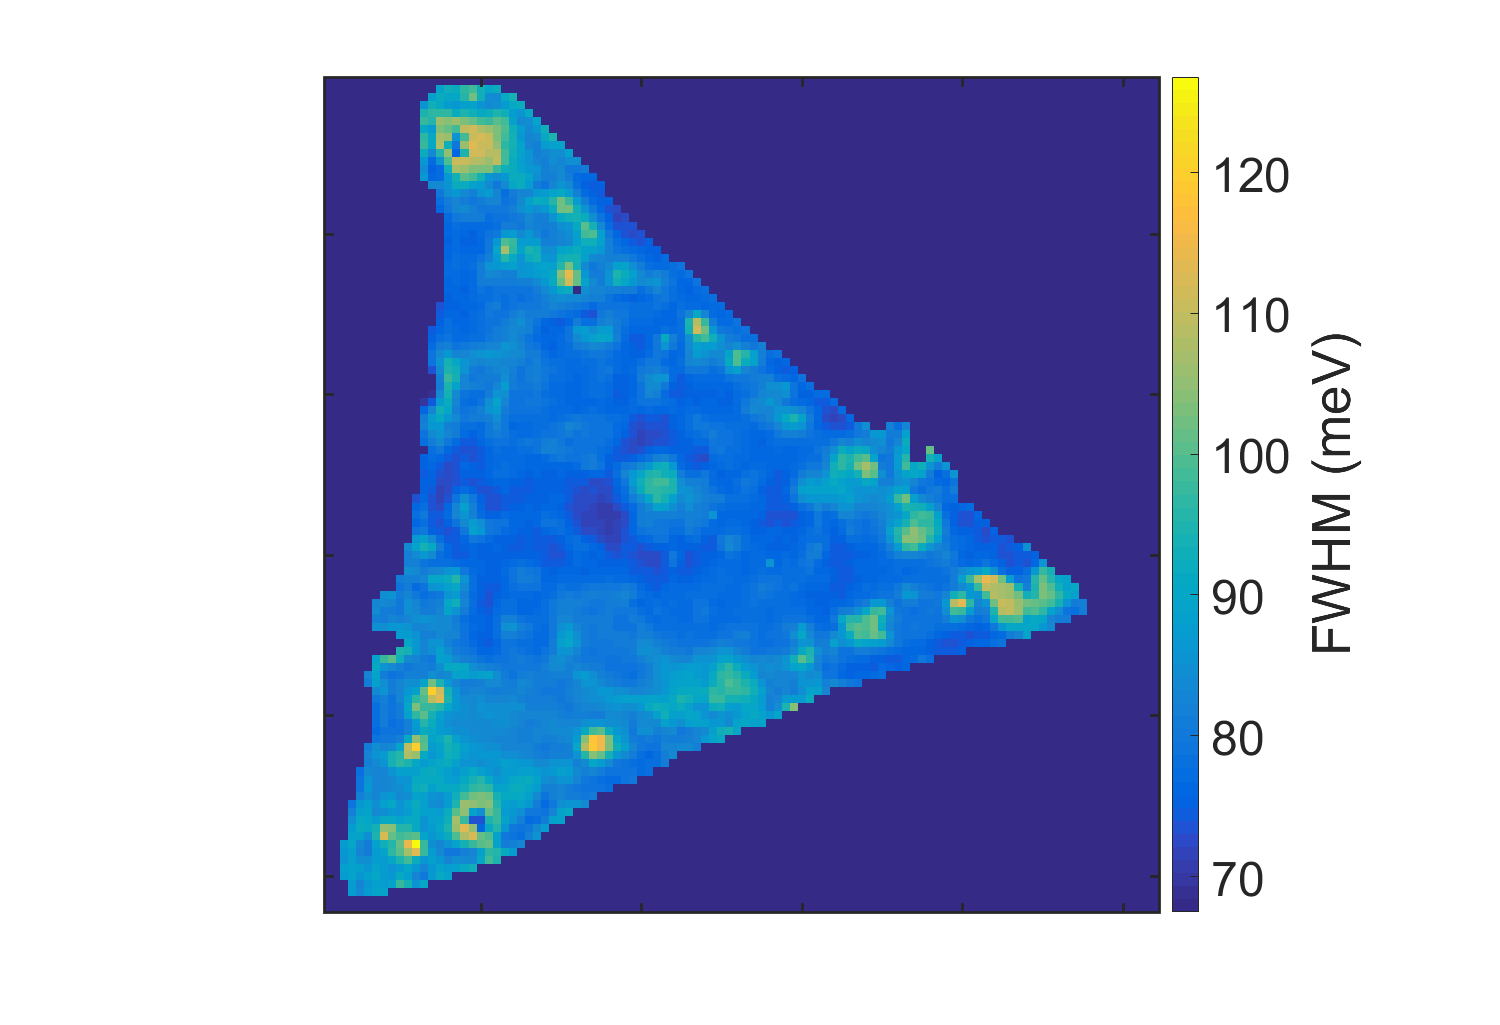
\includegraphics[scale=0.15]{Transfer/TransferPLWidthMapTransferred.png}
			\caption{PL FWHM map of transferred sample}
		\label{fig:TransferPLWidthMapTransferred}
		\end{subfigure}
		\caption{PL spectra maps of samples before and after transfer}
		\label{fig:TransferPLMapsComparison}
	\end{center}
\end{figure}
	
\begin{figure}[H] %Raman Transfer Maps
	\begin{center}
		\begin{subfigure}[b]{0.4\textwidth}
			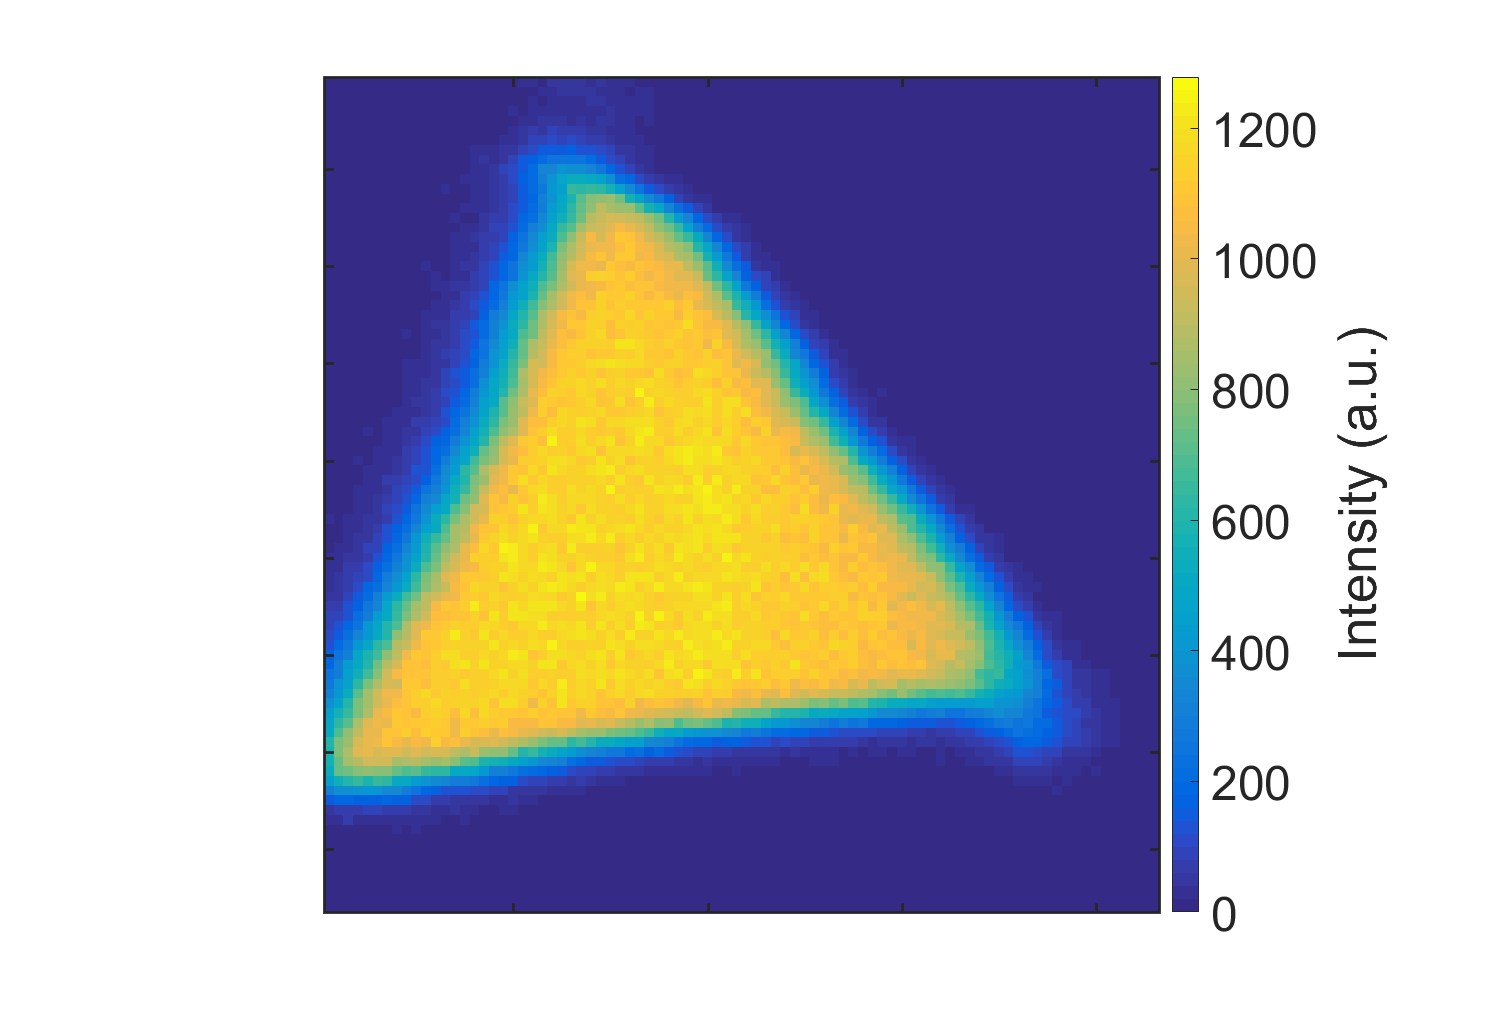
\includegraphics[scale=0.15]{Transfer/TransferRamanIntensityEMapAsgrown.png}
			\caption{Raman $E^1_{2g}$ intensity map of as grown sample}
			\label{fig:TransferRamanIntensityEMapAsgrown}
		\end{subfigure}
		\quad
		\begin{subfigure}[b]{0.4\textwidth}
			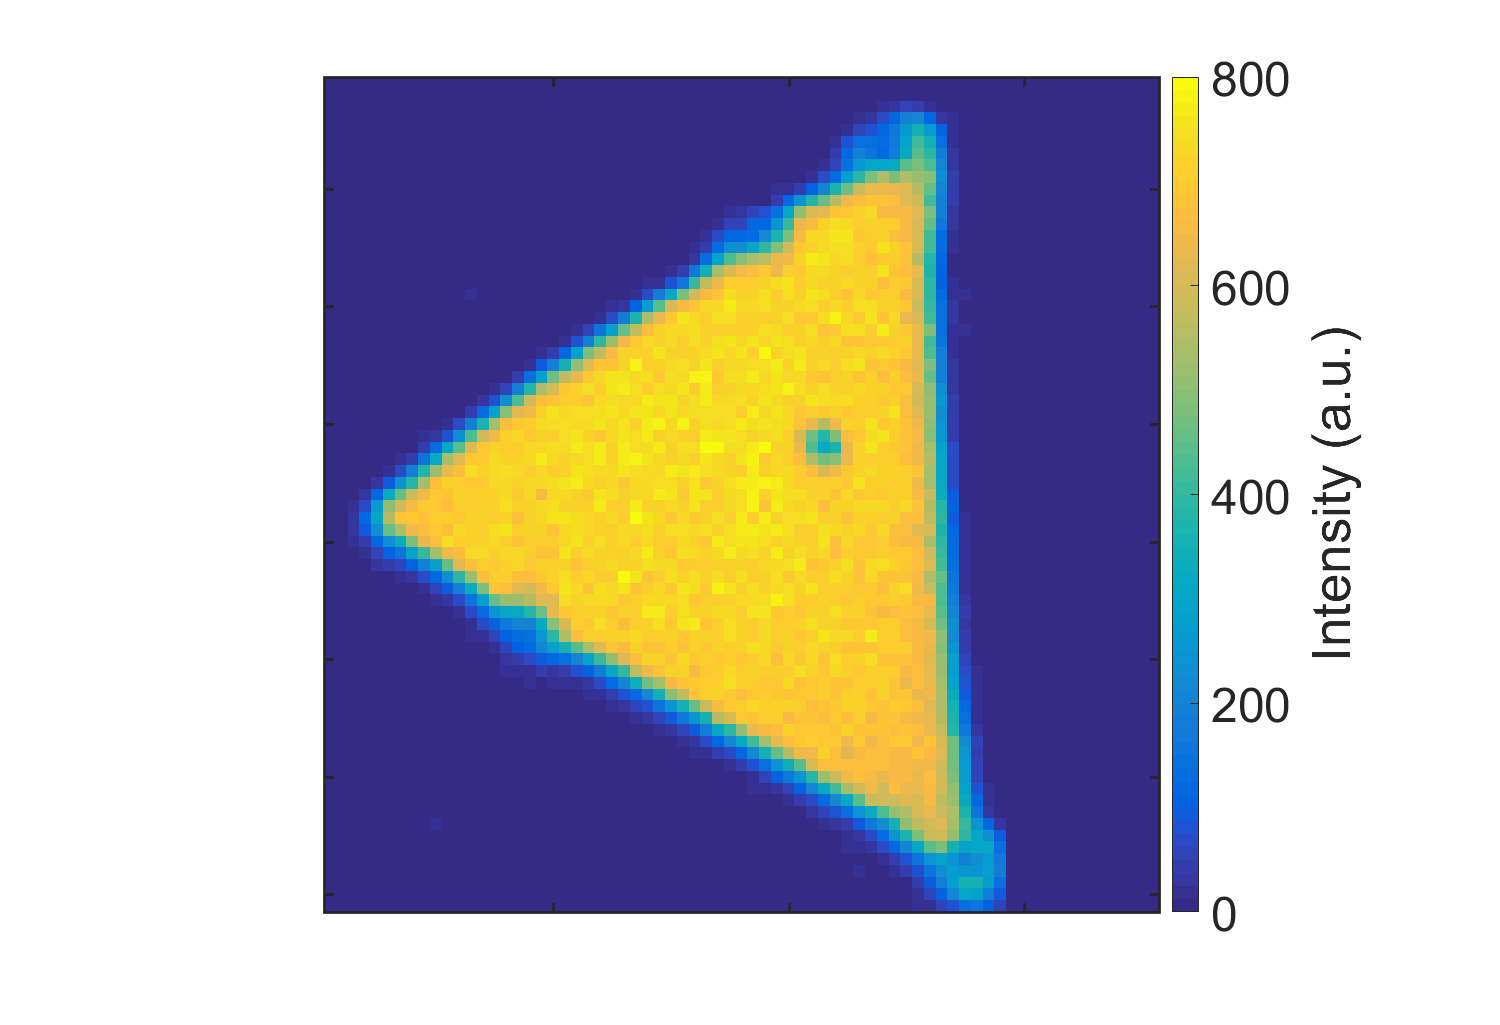
\includegraphics[scale=0.15]{Transfer/TransferRamanIntensityEMapTransferred.png}
			\caption{Raman $E^1_{2g}$ intensity map of transferred sample}
			\label{fig:TransferRamanIntensityMapTransferred}
		\end{subfigure}
		\vfill
		\begin{subfigure}[b]{0.4\textwidth}
			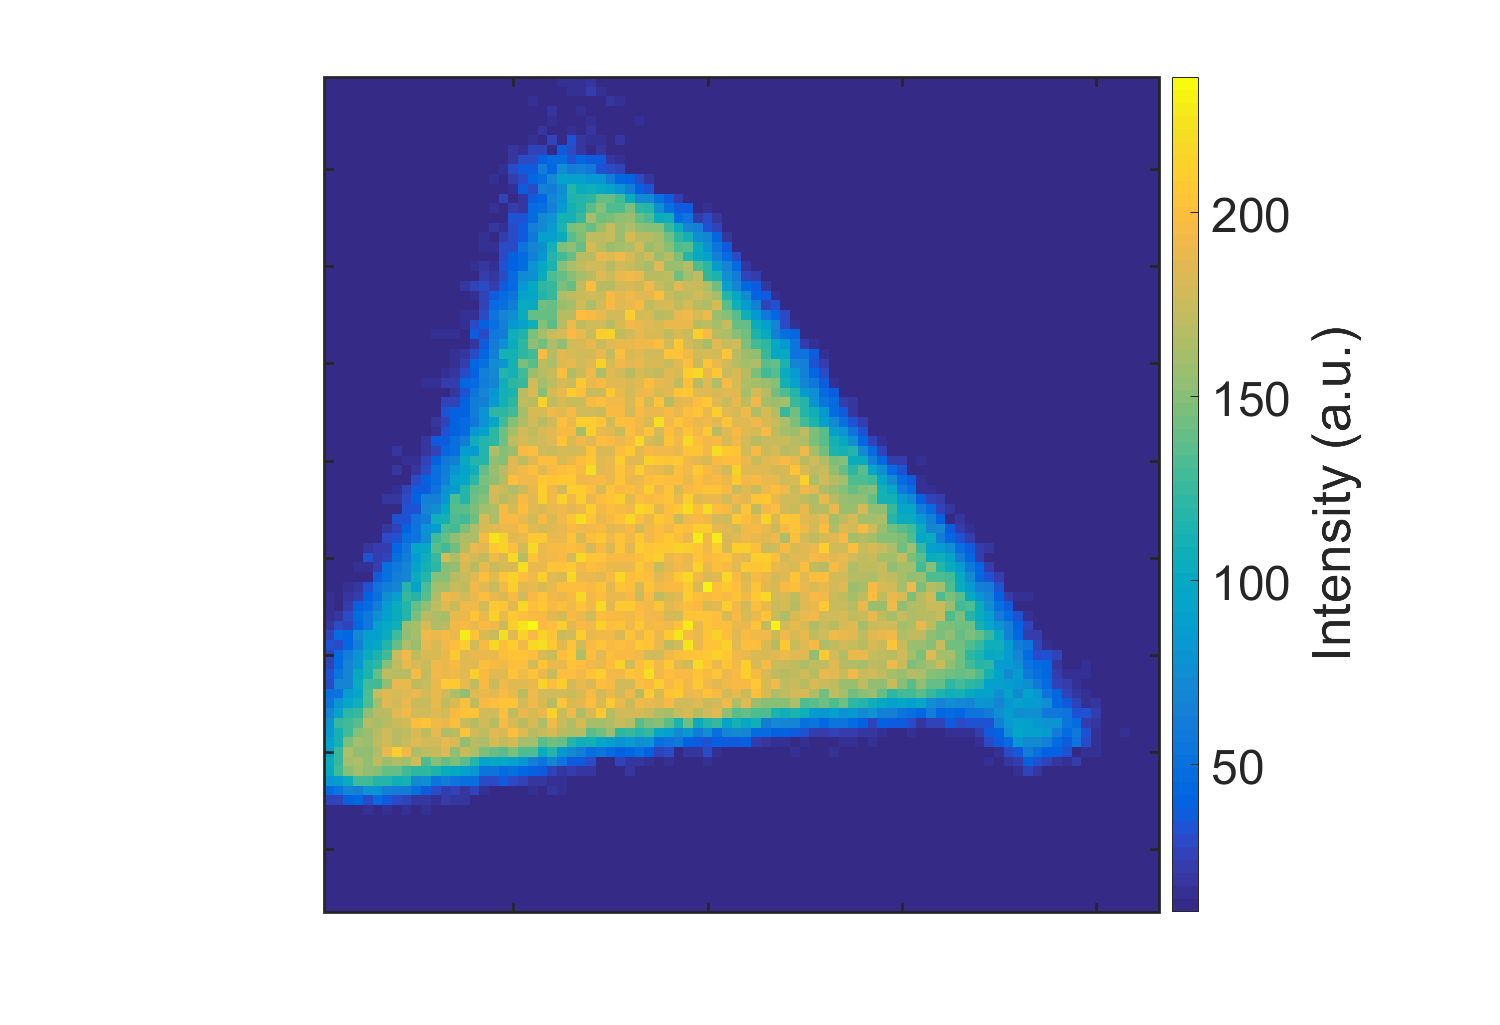
\includegraphics[scale=0.15]{Transfer/TransferRamanIntensityAMapAsgrown.png}
			\caption{Raman $A_{1g}$ intensity map of as grown sample}
			\label{fig:TransferRamanIntensityAMapAsgrown}
		\end{subfigure}
		\quad
		\begin{subfigure}[b]{0.4\textwidth}
			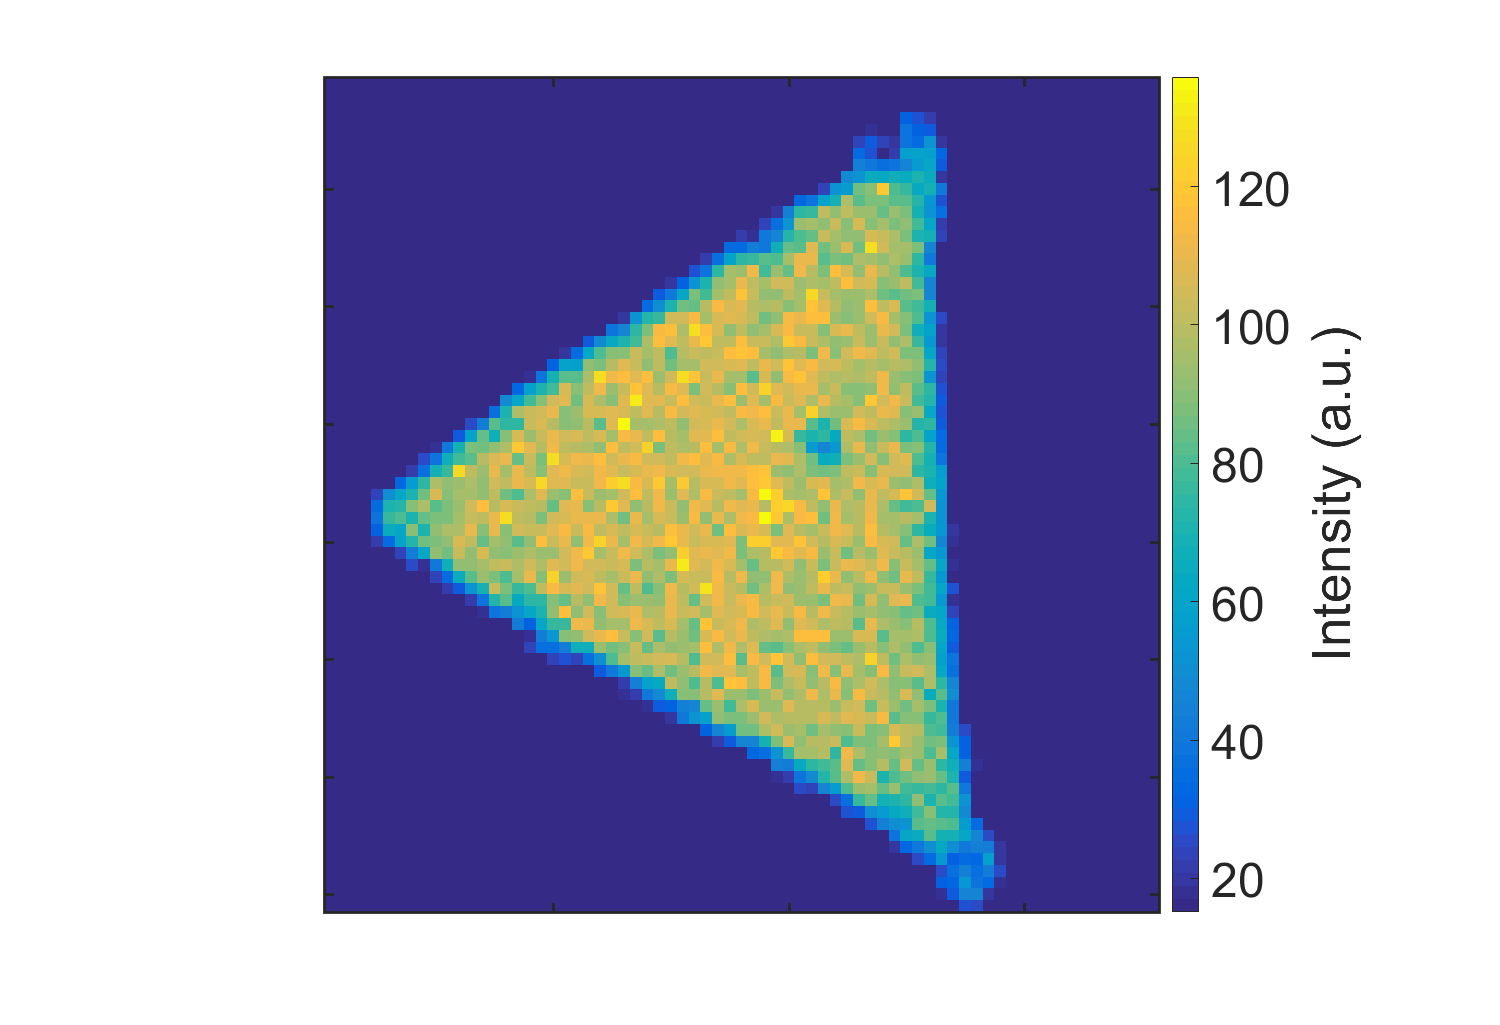
\includegraphics[scale=0.15]{Transfer/TransferRamanIntensityAMapTransferred.png}
			\caption{Raman $A_{1g}$ intensity map of transferred sample}
			\label{fig:TransferRamanIntensityAMapTransferred}
		\end{subfigure}
		\vfill
		\begin{subfigure}[b]{0.4\textwidth}
			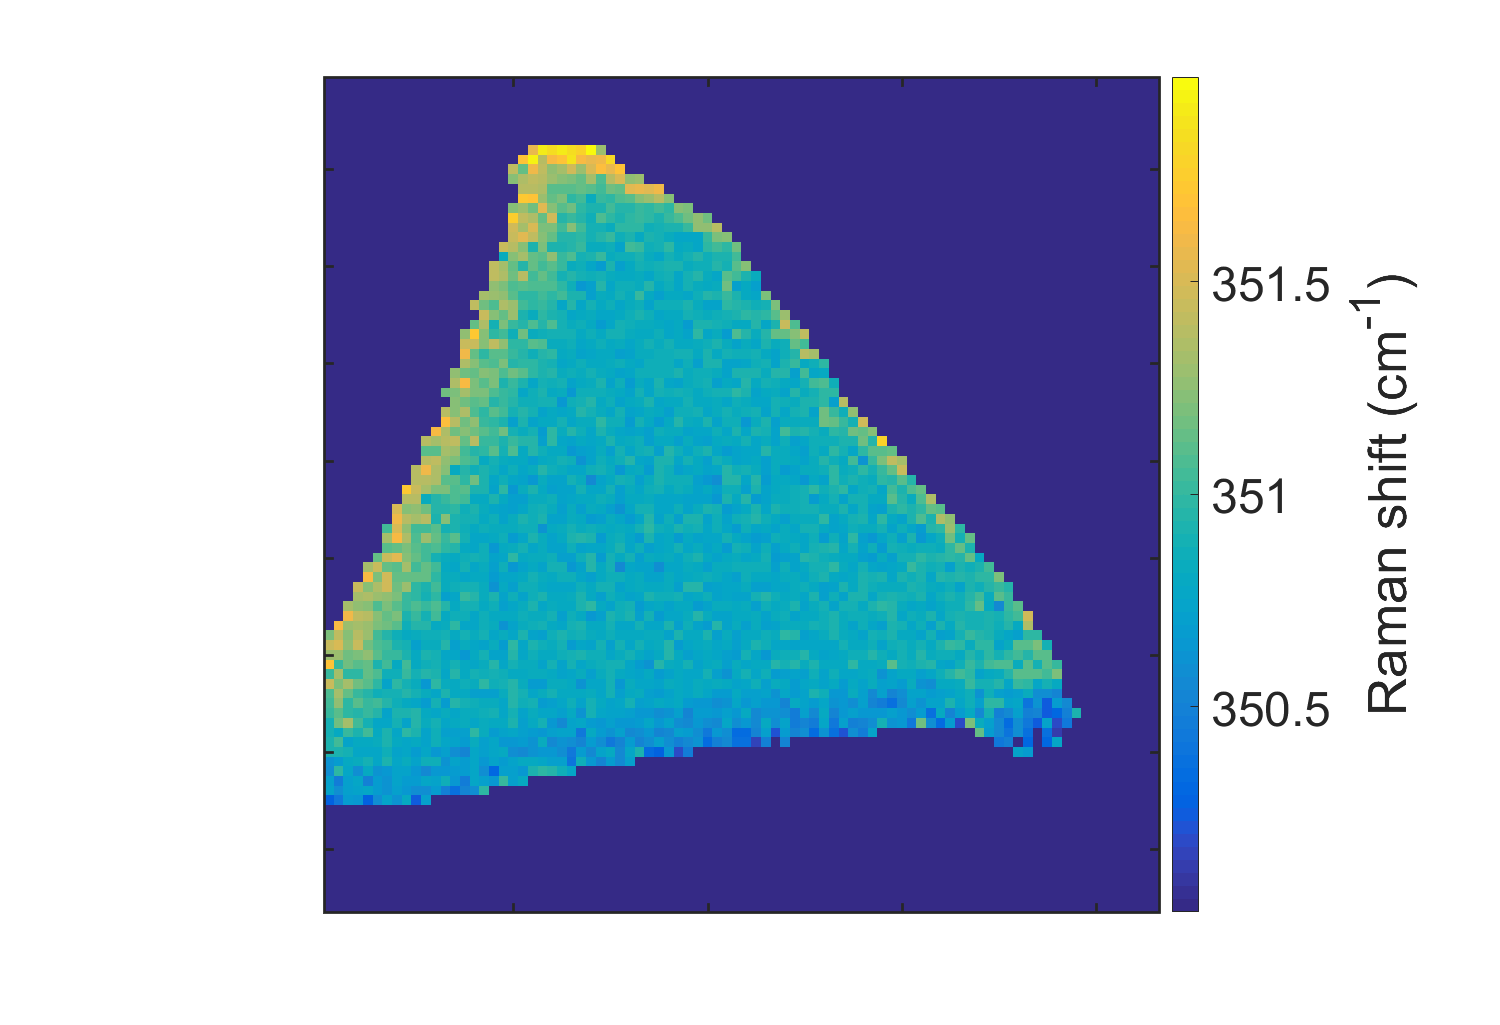
\includegraphics[scale=0.15]{Transfer/TransferRamanPositionEMapAsgrown.png}
			\caption{Raman $E^1_{2g}$ position map of as grown sample}
			\label{fig:TransferRamanPositionEMapAsgrown}
		\end{subfigure}
		\quad
		\begin{subfigure}[b]{0.4\textwidth}
			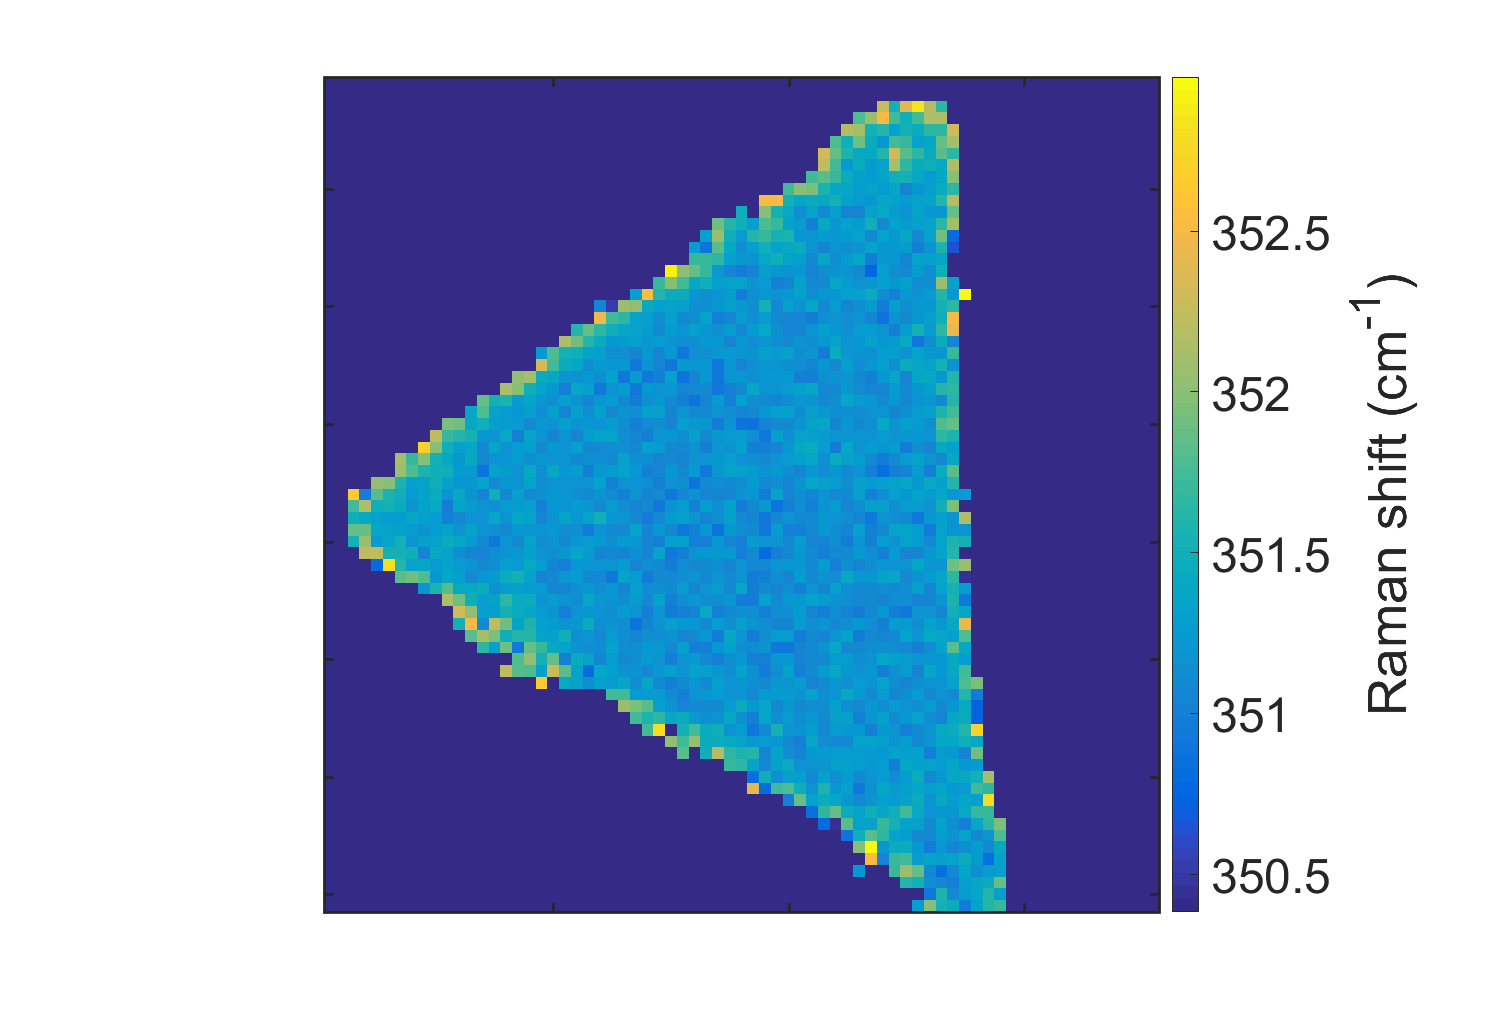
\includegraphics[scale=0.15]{Transfer/TransferRamanPositionEMapTransferred.png}
			\caption{Raman $E^1_{2g}$ position map of transferred sample}
			\label{fig:TransferRamanPositionEMapTransferred}
		\end{subfigure}
		\caption{Raman spectra maps of samples before and after transfer}
		\label{fig:TransferRamanMapsComparison}
	\end{center}
\end{figure}
	
\begin{figure}[H] %Raman Difference and Ratio Transfer Maps
	\begin{center}
		\begin{subfigure}[b]{0.4\textwidth}
			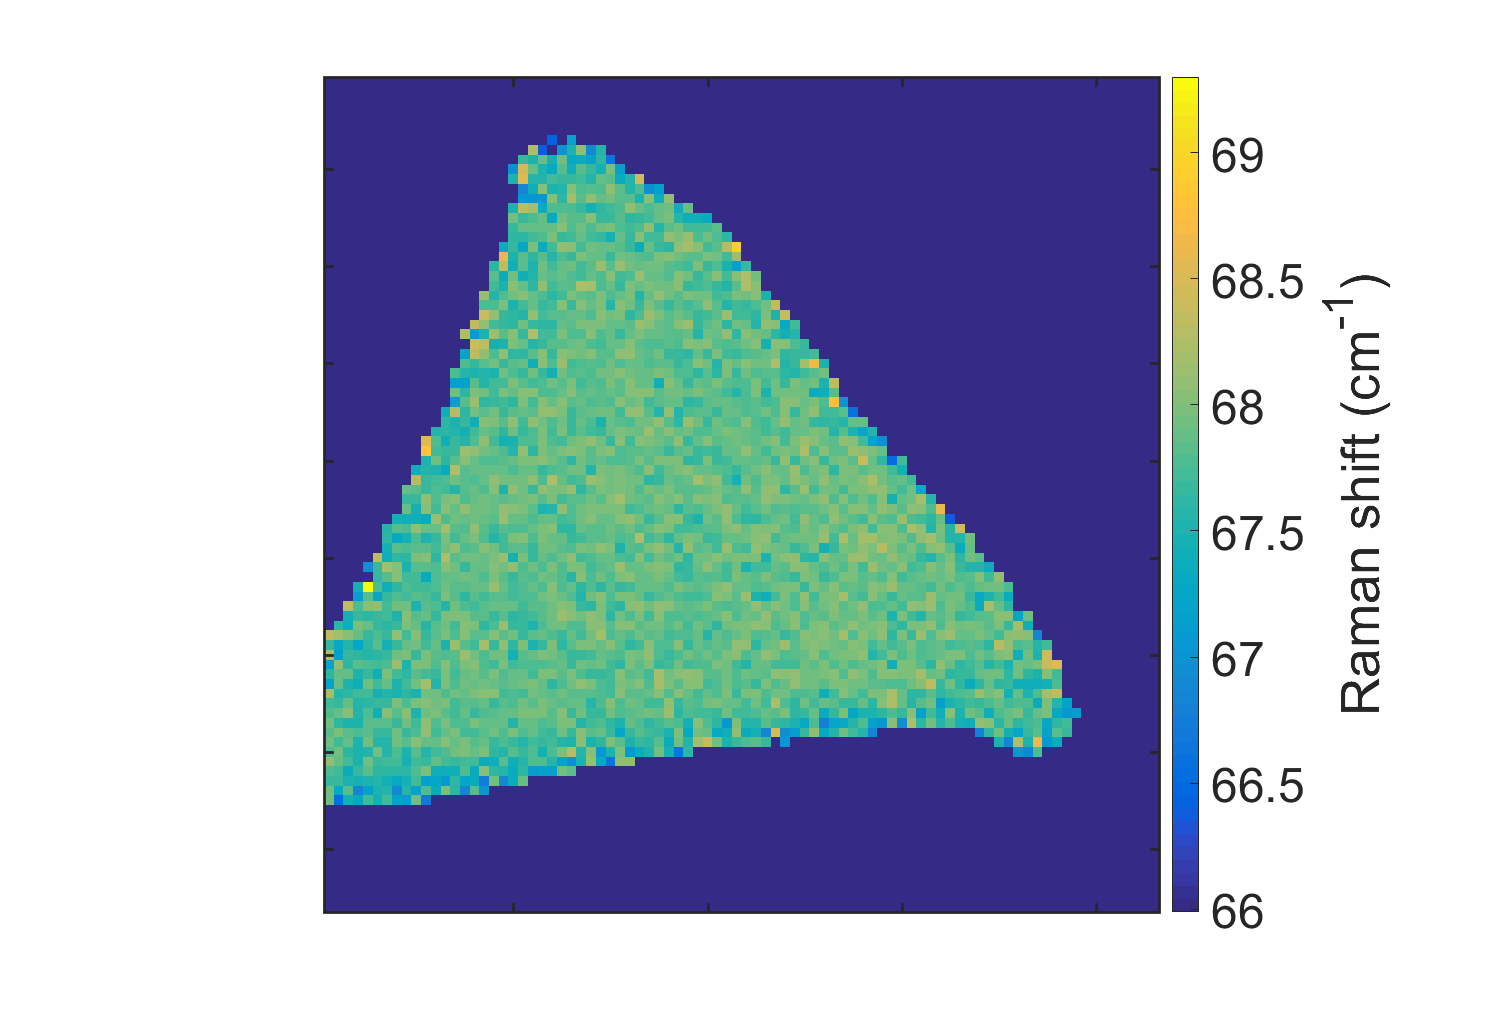
\includegraphics[scale=0.15]{Transfer/TransferRamanDiffMapAsgrown.png}
			\caption{Raman peak position difference map of as grown sample}
			\label{fig:TransferRamanDiffMapAsgrown}
		\end{subfigure}
		\quad
		\begin{subfigure}[b]{0.4\textwidth}
			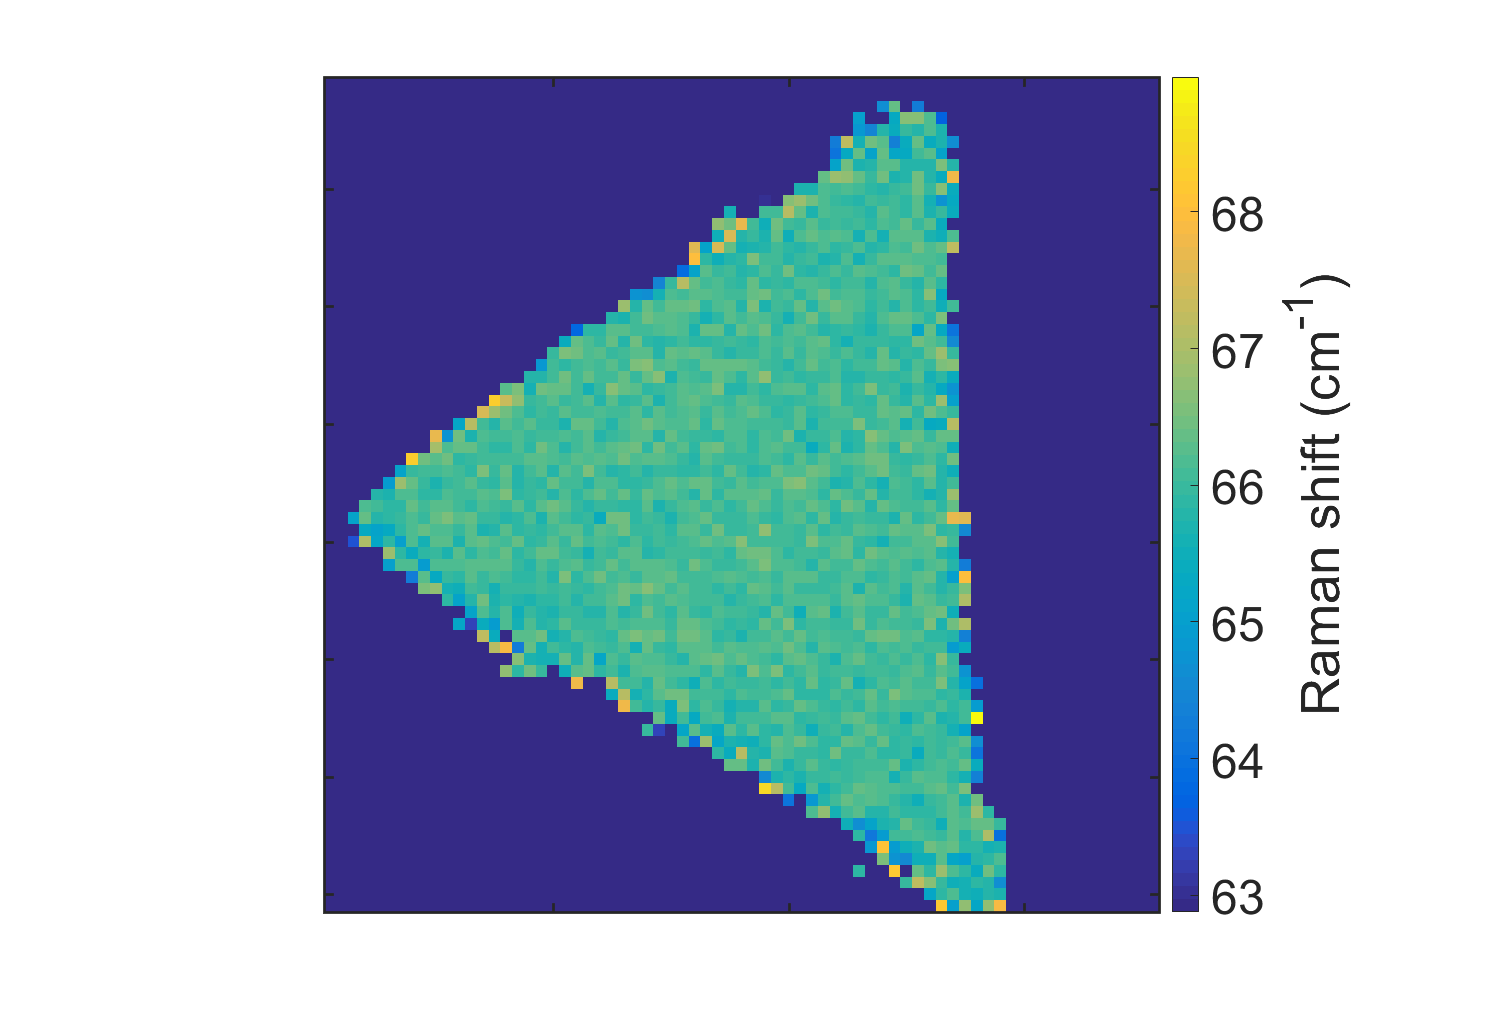
\includegraphics[scale=0.15]{Transfer/TransferRamanDiffMapTransferred.png}
			\caption{Raman peak position difference map of transferred sample}
			\label{fig:TransferRamanDiffMapTransferred}
		\end{subfigure}
		\vfill
		\begin{subfigure}[b]{0.4\textwidth}
			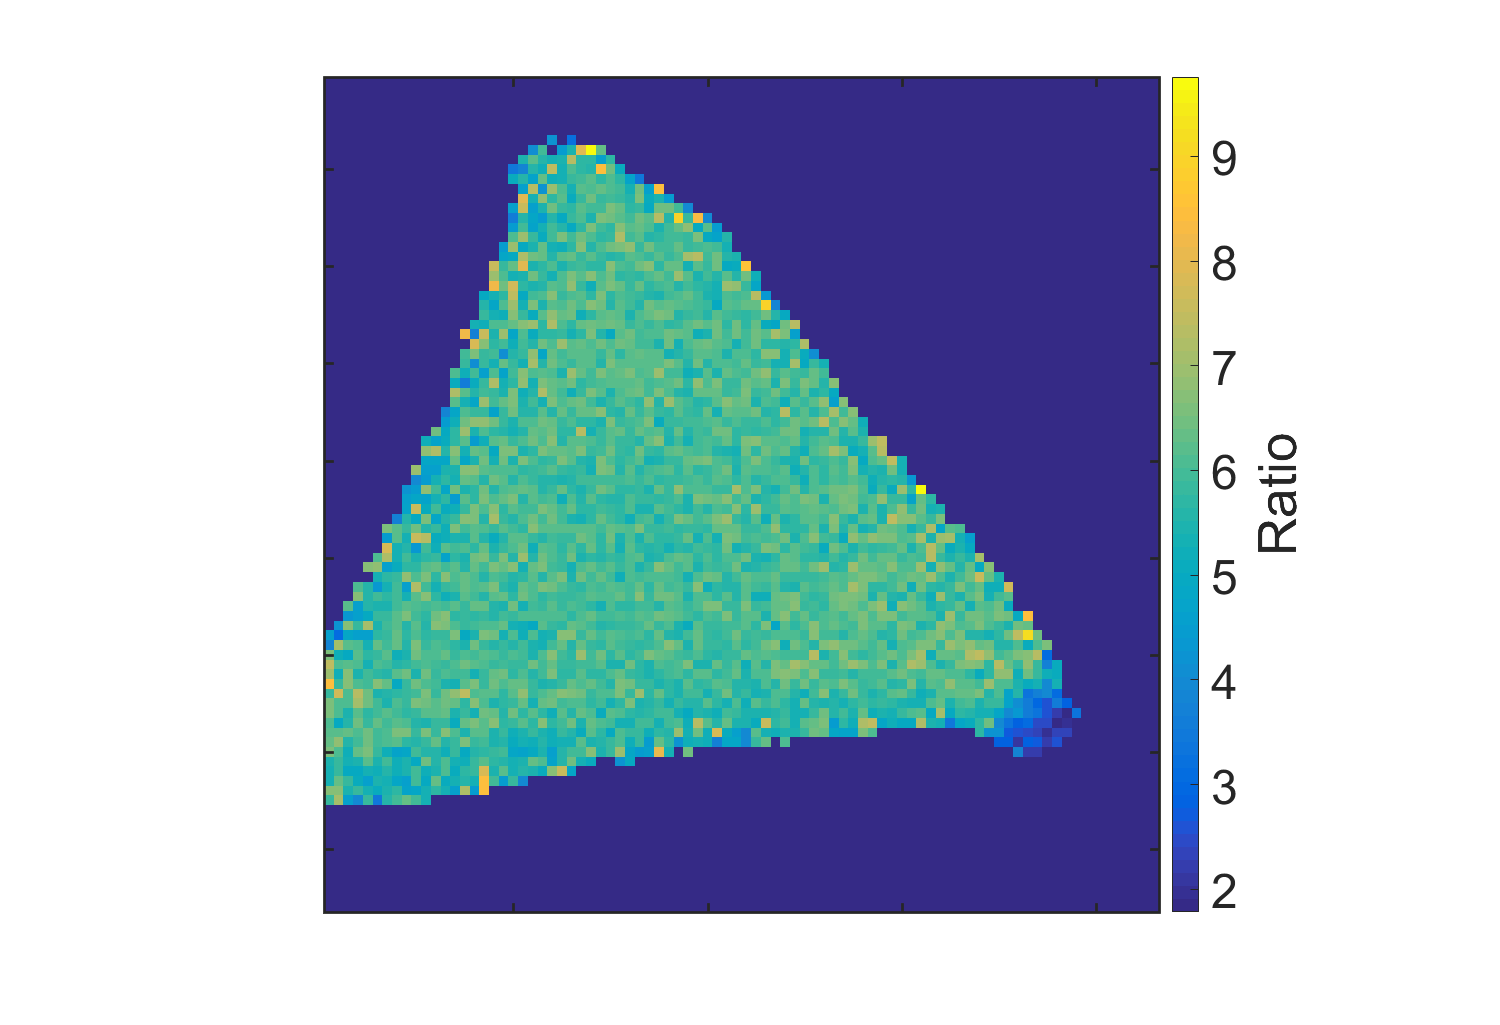
\includegraphics[scale=0.15]{Transfer/TransferRamanRatioMapAsgrown.png}
			\caption{Raman peaks ratio map of as grown sample}
			\label{fig:TransferRamanRatioAMapAsgrown}
		\end{subfigure}
		\quad
		\begin{subfigure}[b]{0.4\textwidth}
			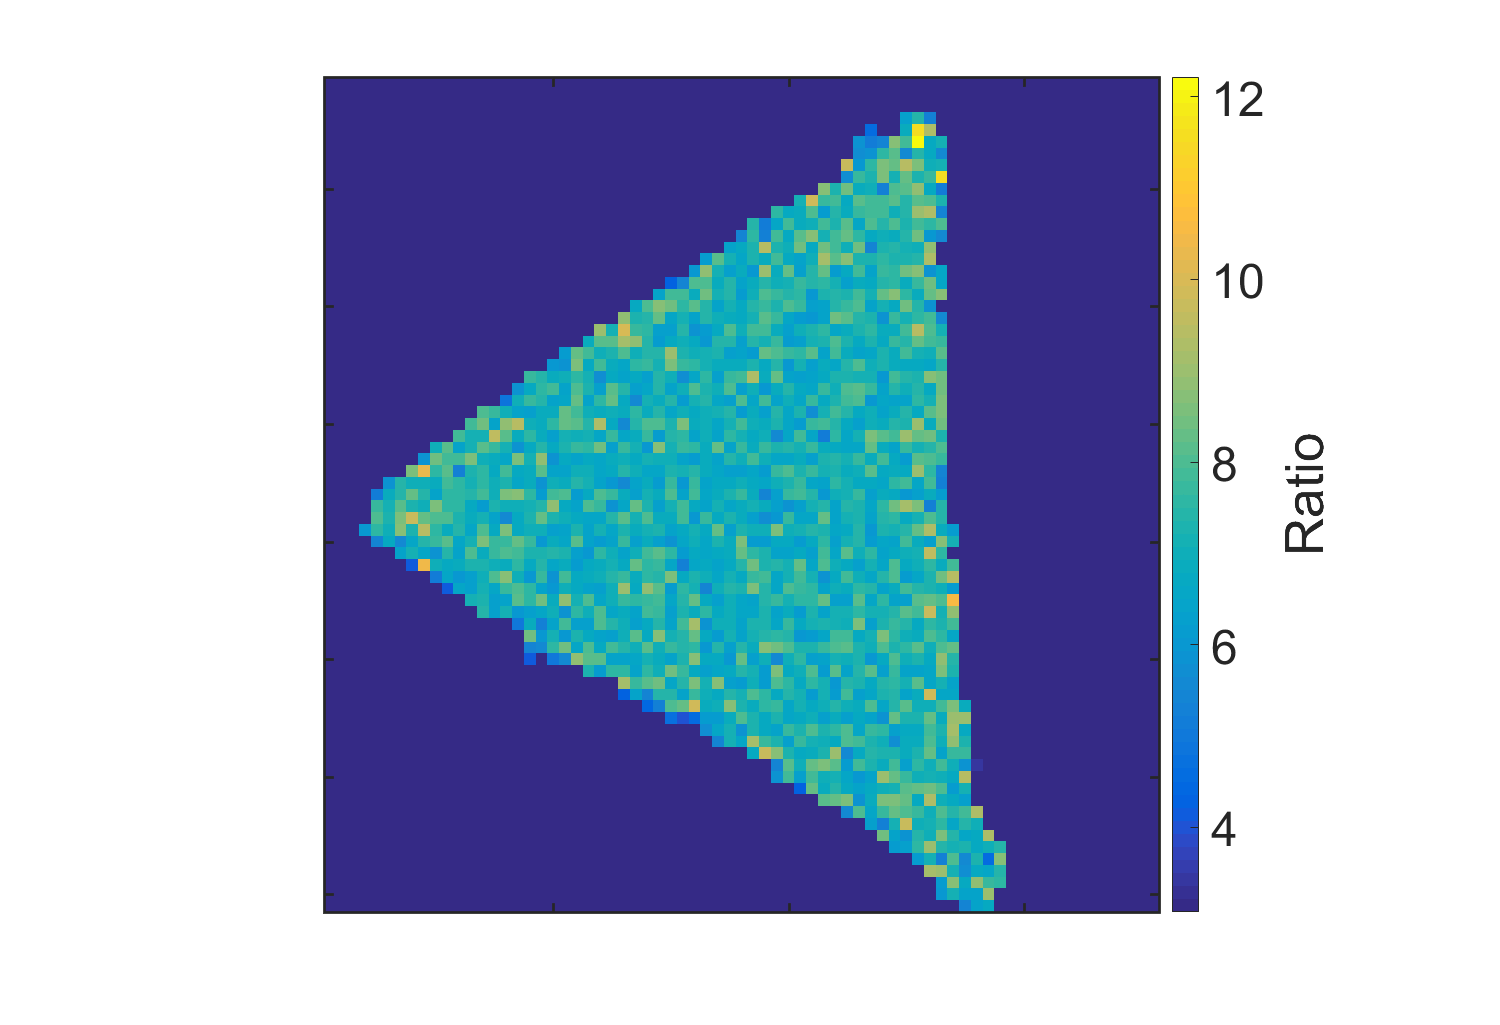
\includegraphics[scale=0.15]{Transfer/TransferRamanRatioMapTransferred.png}
			\caption{Raman peaks ratio map of transferred sample}
			\label{fig:TransferRamanRatioAMapTransferred}
		\end{subfigure}
		\caption{Raman spectra maps of samples before and after transfer}
		\label{fig:TransferRamanDiffRatioMapsComparison}
	\end{center}
\end{figure}
	
\section{Conclusions}
	
In this Chapter we have presented the transfer methodology that we have developed in our own way for monolayer TMDCs. Overall the quality of the transfer material is good and the flakes are pristine in shape. It is unclear to what extent the CVD grown $WS_2$ sample is strained prior to transfer or after it. The difference in relative uncertainty of different fitting parameters of PL and Raman spectra however reveals that the sample becomes less homogeneous following the procedure. This could indicate that a certain degree of strain is introduced as a result of the transfer. This in turn could be attributed to the presence of a non uniform distribution of water molecules, non uniform thickness of PMMA layer, folds in the PMMA layer or presence of residue PMMA.